% TeXstudio spellcheck 2020-12-10 16:39

\chapter{Kiértékelés} \label{esettanulmany}

Ebben a fejezetben a Fischer-protokollon keresztül részletesen bemutatom a megvalósított teljes tesztgenerálási folyamatot (\ref{fischer}. fejezet) és a megoldásomon végzett mérések eredményeit (\ref{meresek}. fejezet).

\section{Fischer-protokoll} \label{fischer}

A tesztgenerálási folyamatot részletesen a Fischer-féle kölcsönös kizárás protokollon keresztül mutatom be. A protokollban minden folyamatnak négy állapota van: \texttt{A} (kezdőállapot), \texttt{req}, \texttt{wait}, \texttt{cs} (critical section).

\subsection{UPPAAL modell} \label{UPPAALmodell}
A Fischer-protokoll UPPAAL modelljében a következő deklarációk találhatók:

\begin{verbatim}
const int N = 2;
typedef int[1, N] id_t;
int id;
\end{verbatim}

A fentiekben az \texttt{N} változóban tároljuk a folyamatok számát, \texttt{id\_t} néven pedig definiálunk egy olyan \texttt{int} típust, amelynek értékkészlete \texttt{[1, N]}, vagyis esetünkben \texttt{[1, 2]}. Definiálunk továbbá egy \texttt{id} nevű, \texttt{int} típusú változót, amely azt fogja tárolni, hogy éppen melyik azonosítójú folyamatunk tartózkodik a kritikus szakaszban (\texttt{cs}).

Az egy folyamatot leíró sablon automatánk neve \texttt{P}, egyetlen paramétere \texttt{const id\_t pid}, a folyamat azonosítója. A sablonban a következő deklarációk találhatók, vagyis a rendszer egyedüli óraváltozója \texttt{x}:

\begin{verbatim}
clock x;
const int a = 32;
const int b = 64;
\end{verbatim}

A sablon automata az \ref{fig:fischer-uppaal}. ábrán látható.

\begin{figure}%[h!]
    \centering
    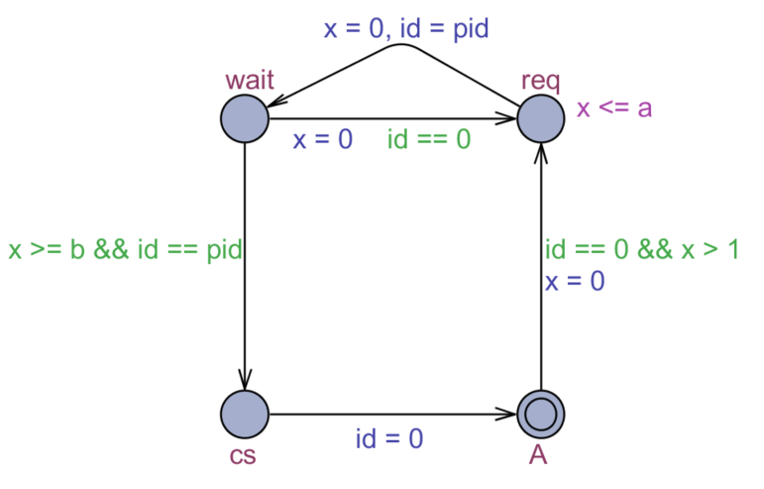
\includegraphics[width=80mm, keepaspectratio]{src/figures/fischer-uppaal.png}
    \caption{A Fischer-protokoll sablon automatája UPPAAL-ban}
    \label{fig:fischer-uppaal}
\end{figure}

\subsection{XTA formalizmus}
Az \ref{UPPAALmodell}. fejezetben bemutatott rendszert a következő XTA fájlba menti az UPPAAL:

\begin{verbatim}
const int N = 2;

typedef int[1, N] id_t;
int id;

process P(const id_t pid) {
clock x;
	const int a = 32;
	const int b = 64;
state
    wait,
    req {x <= a},
    A,
    cs;
init A;
trans
    A -> req { guard id == 0 && x > 1; assign x = 0;  },
    req -> wait { assign x = 0, id = pid;  },
    wait -> req { guard id == 0; assign x = 0;  },
    wait -> cs { guard x >= b && id == pid;  },
    cs -> A { assign id = 0;  };
}
system P;
\end{verbatim}

\subsection{ARG}
A modellből a Theta modellellenőrzője által felépített ARG egy részlete látható az \ref{fig:fischer-arg-reszlet} ábrán, a szaggatott élek az egymást fedő csúcsokat jelölik. (A teljes, 27 csúcsú ARG-t ábrázoló kép akkora, hogy teljesen olvashatatlan lenne.)

\begin{figure}%[h!]
    \centering
    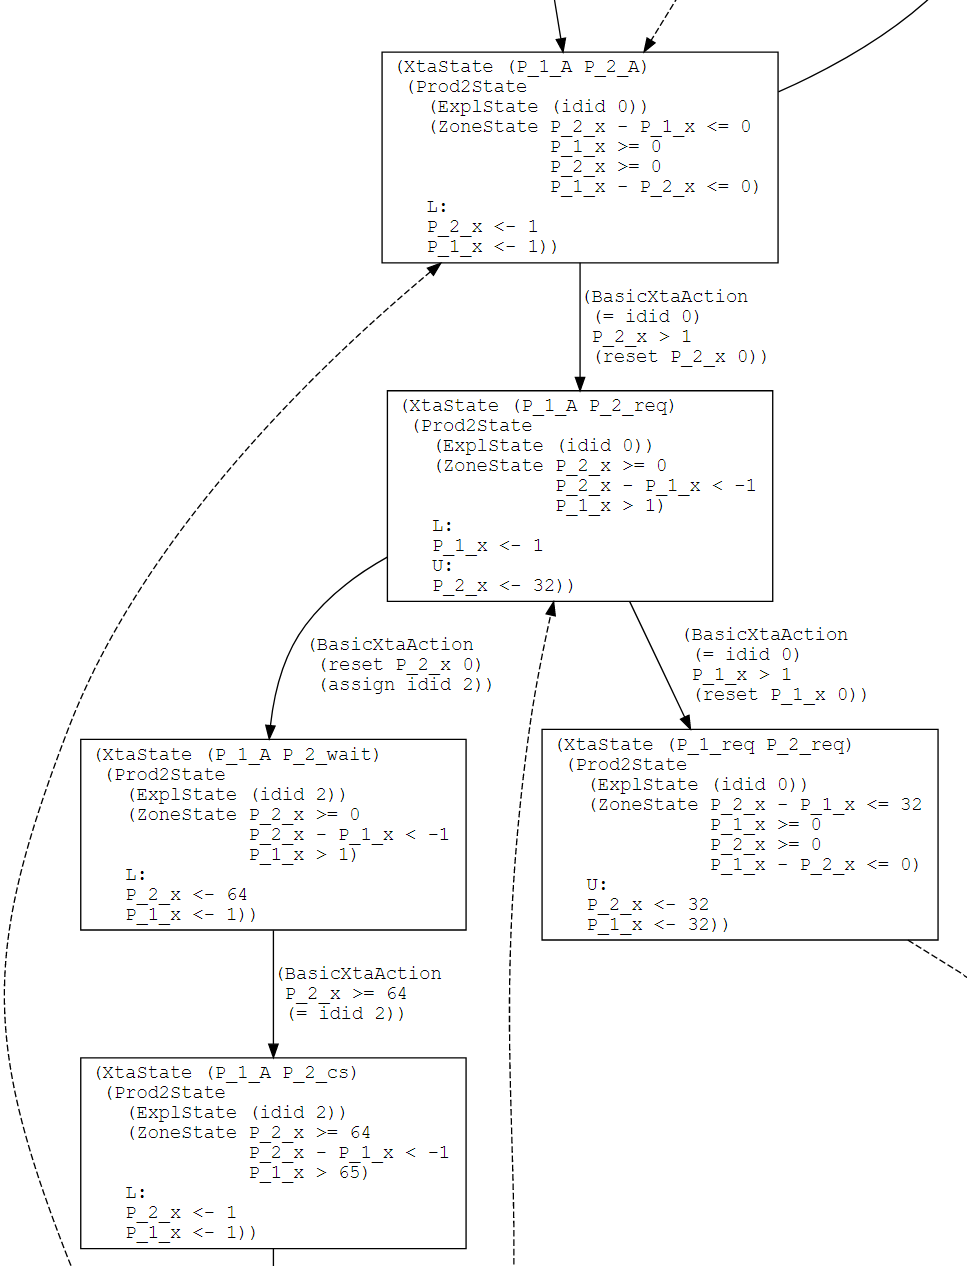
\includegraphics[width=\textwidth, keepaspectratio]{src/figures/fischer-arg-reszlet.png}
    \caption{A kétfolyamatú Fischer-protokoll ARG-jének részlete}
    \label{fig:fischer-arg-reszlet}
\end{figure}

\subsection{Tesztkészlet}

A kétfolyamatú modell összesen 8 vezérlési helyét a tesztgeneráló algoritmus 2 tesztesettel lefedte, ezek láthatók az \ref{fig:fischer-tests}. ábrán.

Megfigyelhető, hogy az \ref{fig:fischer-test1} ábrán látható teszteseten csak a \texttt{P\_1} automata lép, míg a \ref{fig:fischer-test2} ábrán láthatón csak \texttt{P\_2}.

A tört \texttt{delay} értékek magyarázata az \texttt{A} vezérlési helyről \texttt{req} vezérlési helyre vezető élen lévő \texttt{x > 1} őrfeltétel, amely kifejezésnek nincs minimális megoldása.

A tesztesetek szöveges leírása \aref{fig:fischer-tests-text}. ábrán látható.

\begin{figure}
\centering
\begin{minipage}{0.49\textwidth}
{\small \begin{verbatim}========== TRACE__7__P_1_cs ==========
(XtaState (P_1_A P_2_A)
  (Prod2State
    (ExplState (idid 0))
    (ZoneState P_2_x - P_1_x <= 0
               P_1_x >= 0
               P_2_x >= 0
               P_1_x - P_2_x <= 0)
    L:
    P_2_x <- 1
    P_1_x <- 1))
Delay: 1,484375
(BasicXtaAction
  (= idid 0)
  P_1_x > 1
  (reset P_1_x 0))
(XtaState (P_1_req P_2_A)
  (Prod2State
    (ExplState (idid 0))
    (ZoneState P_1_x - P_2_x < -1
               P_2_x > 1
               P_1_x >= 0)
    L:
    P_2_x <- 1
    U:
    P_1_x <- 32))
Delay: 0,000000
(BasicXtaAction
  (reset P_1_x 0)
  (assign idid 1))
(XtaState (P_1_wait P_2_A)
  (Prod2State
    (ExplState (idid 1))
    (ZoneState P_1_x - P_2_x < -1
               P_2_x > 1
               P_1_x >= 0)
    L:
    P_2_x <- 1
    P_1_x <- 64))
Delay: 64,000000
(BasicXtaAction
  (= idid 1)
  P_1_x >= 64)
(XtaState (P_1_cs P_2_A)
  (Prod2State
    (ExplState (idid 1))
    (ZoneState P_1_x - P_2_x < -1
               P_2_x > 65
               P_1_x >= 64)
    L:
    P_2_x <- 1
    P_1_x <- 1))
Delay: 0,000000
Total time: 65,484375
\end{verbatim}}
\subcaption{P\_1 vezérlési helyeit fedő teszteset}
\end{minipage}%
\hspace{0.01\textwidth}
\begin{minipage}{0.49\textwidth}%
%\centering
{\small \begin{verbatim}========== TRACE__10__P_2_cs ==========
(XtaState (P_1_A P_2_A)
  (Prod2State
    (ExplState (idid 0))
    (ZoneState P_2_x - P_1_x <= 0
               P_1_x >= 0
               P_2_x >= 0
               P_1_x - P_2_x <= 0)
    L:
    P_2_x <- 1
    P_1_x <- 1))
Delay: 1,500000
(BasicXtaAction
  (= idid 0)
  P_2_x > 1
  (reset P_2_x 0))
(XtaState (P_1_A P_2_req)
  (Prod2State
    (ExplState (idid 0))
    (ZoneState P_2_x >= 0
               P_2_x - P_1_x < -1
               P_1_x > 1)
    L:
    P_1_x <- 1
    U:
    P_2_x <- 32))
Delay: 0,000000
(BasicXtaAction
  (reset P_2_x 0)
  (assign idid 2))
(XtaState (P_1_A P_2_wait)
  (Prod2State
    (ExplState (idid 2))
    (ZoneState P_2_x >= 0
               P_2_x - P_1_x < -1
               P_1_x > 1)
    L:
    P_2_x <- 64
    P_1_x <- 1))
Delay: 64,000000
(BasicXtaAction
  P_2_x >= 64
  (= idid 2))
(XtaState (P_1_A P_2_cs)
  (Prod2State
    (ExplState (idid 2))
    (ZoneState P_2_x >= 64
               P_2_x - P_1_x < -1
               P_1_x > 65)
    L:
    P_2_x <- 1
    P_1_x <- 1))
Delay: 0,000000
Total time: 65,500000
\end{verbatim}}
\subcaption{P\_2 vezérlési helyeit fedő teszteset}
\end{minipage}
\caption{A kétfolyamatú Fischer-protokoll kettő tesztesete szövegesen}
\label{fig:fischer-tests-text}
\end{figure}

\begin{figure}
     \centering
     \begin{subfigure}[b]{0.4\textwidth}
         \centering
         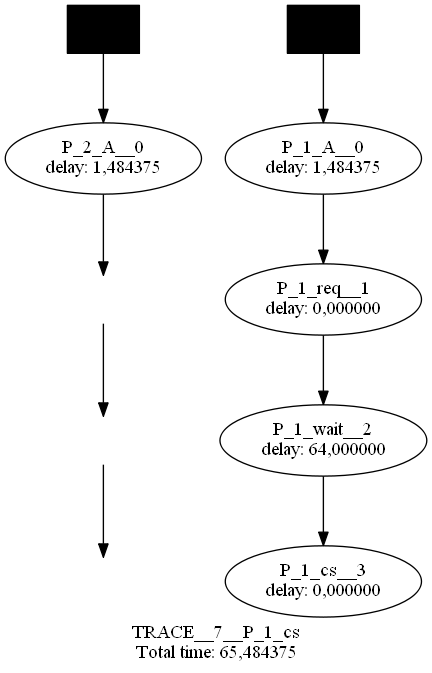
\includegraphics[width=\textwidth]{src/figures/fischer-test1.png}
         \caption{P\_1 vezérlési helyeit fedő teszteset}
         \label{fig:fischer-test1}
     \end{subfigure}
     \hfill
     \begin{subfigure}[b]{0.4\textwidth}
         \centering
         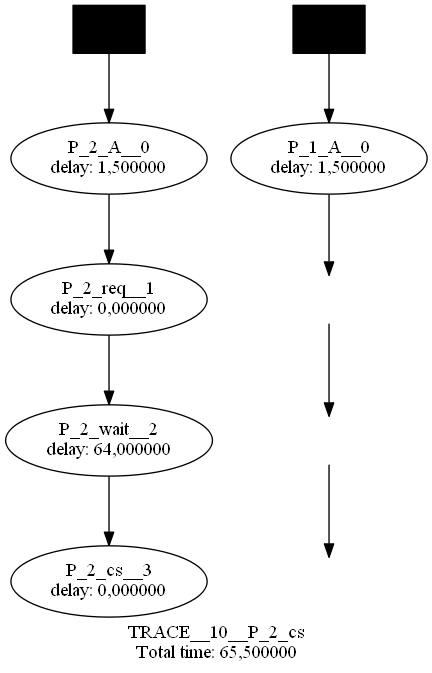
\includegraphics[width=\textwidth]{src/figures/fischer-test2.png}
         \caption{P\_2 vezérlési helyeit fedő teszteset}
         \label{fig:fischer-test2}
     \end{subfigure}
        \caption{A kétfolyamatú Fischer-protokoll kettő tesztesete grafikusan}
        \label{fig:fischer-tests}
\end{figure}

\section{Mérések} \label{meresek}

A bemutatott tesztgenerálási algoritmust számos XTA modellen lemértem. A mérések során a tesztgenerálás futásidejét, a generált tesztek számát, valamint a végső tesztkészlet elemszámát és a benne lévő tesztek összesített hosszát vizsgáltam.

A mérések során a Theta-t a \texttt{-{}-clock LU -{}-search BFS} paraméterekkel futtattam, minden tesztesetet 60 másodperces időkorláttal (ez az időkorlát nem a tesztgenerálásra, hanem a teljes futásra értendő). A méréseket Windows 10 operációs rendszeren végeztem, Intel Core i5-7200 processzorral, 8 GB RAM-mal. A mérési eredmények \aref{table:meresek}. táblázatban láthatók.

\begin{table}
\centering
\begin{tabular}{ |c||c|c||c|c|c|c| } 
 \hline
 \multirow{2}{*}{Modell} & \multicolumn{2}{c||}{ARG} & \multirow{2}{*}{\makecell{Futásidő \\ (ms)}} & \multirow{2}{*}{\makecell{Generált \\ tesztek}} & \multirow{2}{*}{$|\networktestset|$} & \multirow{2}{*}{$\sum{|\networktestset_i|}$} \\
  & mélység & méret & & & & \\
 
 \hline
critical-01-25-50.xta & 7 & 27 & 274 & 12 & 2 & 13 \\
critical-02-25-50.xta & 14 & 641 & 1723 & 85 & 4 & 28 \\
critical-03-25-50.xta & 22 & 21699 & 7623 & 410 & 6 & 45 \\
\hline
csma-01.xta & 2 & 3 & 509 & 2 & 1 & 2 \\
csma-02.xta & 5 & 21 & 353 & 9 & 2 & 7 \\
csma-03.xta & 8 & 99 & 1306 & 18 & 4 & 13 \\
csma-04.xta & 9 & 381 & 875 & 24 & 6 & 19 \\
csma-05.xta & 10 & 1272 & 1723 & 40 & 7 & 21 \\
csma-06.xta & 11 & 3865 & 2040 & 53 & 9 & 25 \\
csma-07.xta & 12 & 11008 & 4488 & 93 & 12 & 33 \\
csma-08.xta & 13 & 29925 & 4264 & 100 & 13 & 37 \\
csma-09.xta & 14 & 78552 & 4278 & 119 & 16 & 44 \\
\hline
fddi-001.xta & 9 & 15 & 813 & 11 & 2 & 15 \\
fddi-002.xta & 16 & 46 & 2144 & 26 & 3 & 34 \\
fddi-003.xta & 24 & 104 & 8495 & 48 & 4 & 60 \\
fddi-004.xta & 28 & 101 & 18073 & 62 & 4 & 74 \\
fddi-005.xta & 34 & 141 & 52396 & 85 & 4 & 89 \\
\arrayrulecolor{red}\hdashline\arrayrulecolor{black}
\textcolor{red}{fddi-006.xta} & \multicolumn{6}{c|}{\textcolor{red}{időtúllépés}} \\
\hline
fischer-01-32-64.xta & 4 & 5 & 152 & 4 & 1 & 4 \\
fischer-02-32-64.xta & 8 & 27 & 380 & 10 & 2 & 8 \\
fischer-03-32-64.xta & 10 & 121 & 508 & 20 & 3 & 12 \\
fischer-04-32-64.xta & 12 & 493 & 1083 & 35 & 4 & 16 \\
fischer-05-32-64.xta & 14 & 1911 & 1866 & 56 & 5 & 20 \\
fischer-06-32-64.xta & 16 & 7183 & 2648 & 79 & 6 & 24 \\
fischer-07-32-64.xta & 18 & 26405 & 3294 & 104 & 7 & 28 \\
fischer-08-32-64.xta & 20 & 95353 & 5829 & 165 & 8 & 32 \\
\hline
lynch-01-16.xta & 9 & 10 & 296 & 9 & 1 & 9 \\
lynch-02-16.xta & 13 & 61 & 867 & 30 & 2 & 18 \\
lynch-03-16.xta & 15 & 271 & 1716 & 76 & 3 & 27 \\
lynch-04-16.xta & 17 & 1049 & 4395 & 208 & 4 & 36 \\
lynch-05-16.xta & 19 & 3811 & 13247 & 582 & 5 & 45 \\
lynch-06-16.xta & 21 & 13453 & 39038 & 1490 & 6 & 54 \\
\arrayrulecolor{red}\hdashline\arrayrulecolor{black}
\textcolor{red}{lynch-07-16.xta} & \multicolumn{6}{c|}{\textcolor{red}{időtúllépés}} \\
\textcolor{red}{lynch-08-16.xta} & \multicolumn{6}{c|}{\textcolor{red}{időtúllépés}} \\
\hline
\end{tabular}
\caption{A tesztgenerálási algoritmus mérési eredményei}
\label{table:meresek}
\end{table}